\def\QRCODE{TB_IPR_TUT.IMG.granulometry_matlabqrcode.png}
\def\QRPAGE{http://www.iptutorials.science/tree/master/TB_IPR/TUT.IMG.granulometry/matlab}

\mcorrectionsection{Matlab correction}

\subsection{Morphological granulometry}
The code is straightforward from the definition. It consists on a loop over the different sizes of the structuring element. 
\begin{matlab}
% read image
A=imread('simulation.bmp');
A=logical(double(A)/255);

% visualisation
figure;imshow(A);
title('Original simulated image');
\end{matlab}

Different structuring elements shapes can be used, the most classical one being the disk. In order to suppress small objects, the function \minline{imreconstruct} is used \iflabelexists{tut:binarymorpho:enonce}{(see tutorial \ref{tut:binarymorpho:enonce}).}{(see tutorial on morphological reconstruction).}
\begin{matlab}
% maximal radius size
N=35;

% array of areas and numbers 
areas=zeros(N, 1);
number=zeros(N,1);
area0=sum(A(:));
nbre0=bweuler(A);
% loop over the different sizes
for i=0:N
   se = strel('disk', i, 0); % structuring element
   C = imopen(A, se);        % 
   C = imreconstruct(C,A);   % suppress small objects
   areas(i) = sum(C(:))/area0*100;  % normalized area
   number(i)=bweuler(C)/nbre0*100;% Euler number
end
\end{matlab}
The results are displayed using the following commands, and reproduced in Fig. \ref{fig:granulometry:matlab:granulo}. The function \minline{diff} is used to evaluate a discrete derivative.

\begin{matlab}
% display the results
figure;
subplot(121);plot(0:N,areas,'-xr');title('Granulometry');
hold on; plot(0:N,number,'-xb');legend('area analysis','number analysis');
% finite difference analysis
diff_areas = -diff(areas);
diff_number = -diff(number);
subplot(122);
plot(0:N-1,diff_areas,'-xr');title('Finite differences');
hold on; plot(0:N-1,diff_number,'-xb');
legend('area analysis','number analysis');
\end{matlab}

\begin{figure}[htbp]
\centering
 % This file was created by matlab2tikz v0.4.7 running on MATLAB 8.3.
% Copyright (c) 2008--2014, Nico Schlömer <nico.schloemer@gmail.com>
% All rights reserved.
% Minimal pgfplots version: 1.3
% 
% The latest updates can be retrieved from
%   http://www.mathworks.com/matlabcentral/fileexchange/22022-matlab2tikz
% where you can also make suggestions and rate matlab2tikz.
% 
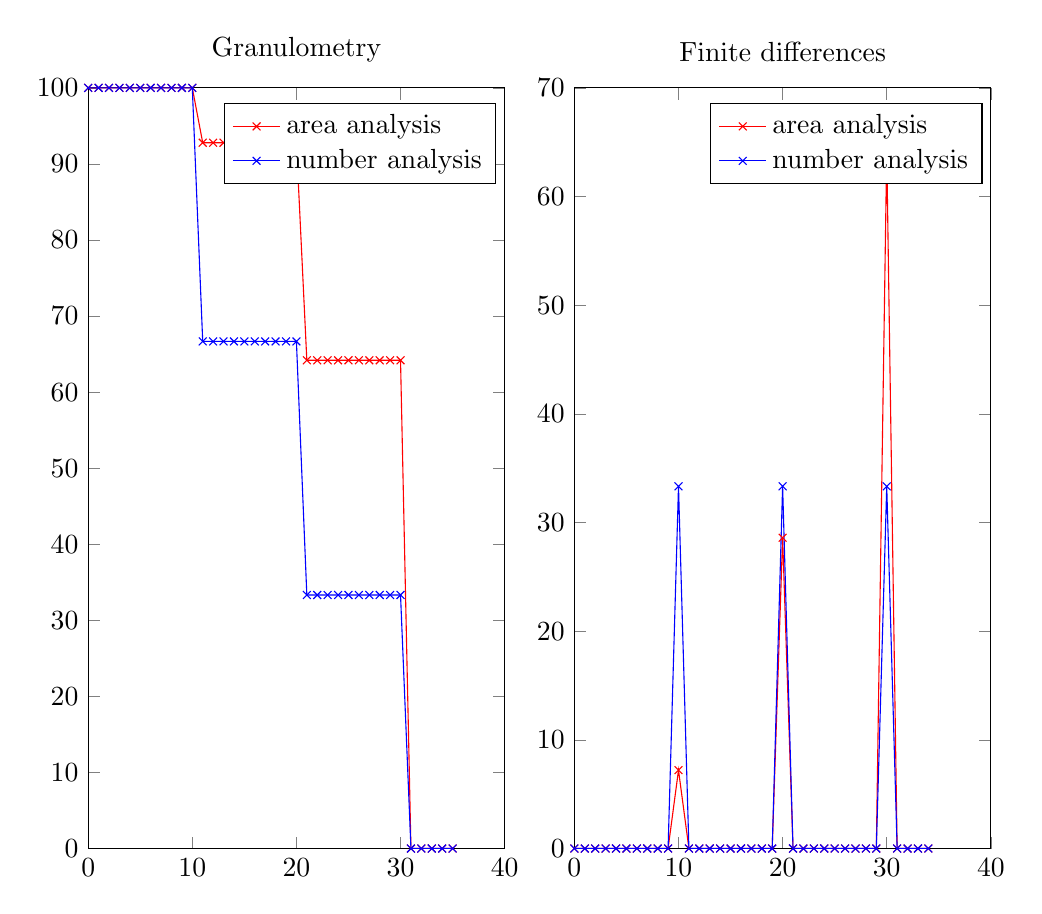
\begin{tikzpicture}

\begin{axis}[%
width=2.08232323232323in,
height=3.80333333333333in,
scale only axis,
xmin=0,
xmax=40,
ymin=0,
ymax=100,
name=plot1,
title={Granulometry},
legend style={draw=black,fill=white,legend cell align=left}
]
\addplot [color=red,solid,mark=x,mark options={solid}]
  table[row sep=crcr]{%
0	100\\
1	100\\
2	100\\
3	100\\
4	100\\
5	100\\
6	100\\
7	100\\
8	100\\
9	100\\
10	100\\
11	92.7872582480091\\
12	92.7872582480091\\
13	92.7872582480091\\
14	92.7872582480091\\
15	92.7872582480091\\
16	92.7872582480091\\
17	92.7872582480091\\
18	92.7872582480091\\
19	92.7872582480091\\
20	92.7872582480091\\
21	64.1865756541524\\
22	64.1865756541524\\
23	64.1865756541524\\
24	64.1865756541524\\
25	64.1865756541524\\
26	64.1865756541524\\
27	64.1865756541524\\
28	64.1865756541524\\
29	64.1865756541524\\
30	64.1865756541524\\
31	0\\
32	0\\
33	0\\
34	0\\
35	0\\
};
\addlegendentry{area analysis};

\addplot [color=blue,solid,mark=x,mark options={solid}]
  table[row sep=crcr]{%
0	100\\
1	100\\
2	100\\
3	100\\
4	100\\
5	100\\
6	100\\
7	100\\
8	100\\
9	100\\
10	100\\
11	66.6666666666667\\
12	66.6666666666667\\
13	66.6666666666667\\
14	66.6666666666667\\
15	66.6666666666667\\
16	66.6666666666667\\
17	66.6666666666667\\
18	66.6666666666667\\
19	66.6666666666667\\
20	66.6666666666667\\
21	33.3333333333333\\
22	33.3333333333333\\
23	33.3333333333333\\
24	33.3333333333333\\
25	33.3333333333333\\
26	33.3333333333333\\
27	33.3333333333333\\
28	33.3333333333333\\
29	33.3333333333333\\
30	33.3333333333333\\
31	0\\
32	0\\
33	0\\
34	0\\
35	0\\
};
\addlegendentry{number analysis};

\end{axis}

\begin{axis}[%
width=2.08232323232323in,
height=3.80333333333333in,
scale only axis,
xmin=0,
xmax=40,
ymin=-0,
ymax=70,
at=(plot1.right of south east),
anchor=left of south west,
title={Finite differences},
legend style={draw=black,fill=white,legend cell align=left}
]
\addplot [color=red,solid,mark=x,mark options={solid}]
  table[row sep=crcr]{%
0	-0\\
1	-0\\
2	-0\\
3	-0\\
4	-0\\
5	-0\\
6	-0\\
7	-0\\
8	-0\\
9	-0\\
10	7.2127417519909\\
11	-0\\
12	-0\\
13	-0\\
14	-0\\
15	-0\\
16	-0\\
17	-0\\
18	-0\\
19	-0\\
20	28.6006825938566\\
21	-0\\
22	-0\\
23	-0\\
24	-0\\
25	-0\\
26	-0\\
27	-0\\
28	-0\\
29	-0\\
30	64.1865756541524\\
31	-0\\
32	-0\\
33	-0\\
34	-0\\
};
\addlegendentry{area analysis};

\addplot [color=blue,solid,mark=x,mark options={solid}]
  table[row sep=crcr]{%
0	-0\\
1	-0\\
2	-0\\
3	-0\\
4	-0\\
5	-0\\
6	-0\\
7	-0\\
8	-0\\
9	-0\\
10	33.3333333333333\\
11	-0\\
12	-0\\
13	-0\\
14	-0\\
15	-0\\
16	-0\\
17	-0\\
18	-0\\
19	-0\\
20	33.3333333333333\\
21	-0\\
22	-0\\
23	-0\\
24	-0\\
25	-0\\
26	-0\\
27	-0\\
28	-0\\
29	-0\\
30	33.3333333333333\\
31	-0\\
32	-0\\
33	-0\\
34	-0\\
};
\addlegendentry{number analysis};

\end{axis}
\end{tikzpicture}%
 \caption{Granulometry and finite differences for the synthetic image of disks.}
 \label{fig:granulometry:matlab:granulo}
\end{figure}

\subsection{Real application}
The code is exactly the same as the previous one, taking a binary image as input. The powder image is segmented using a threshold at value 74, and applying some filtering processes (see result in Fig. \ref{fig:granulometry:matlab:segmented}).

\begin{matlab}
B=imread('poudre.bmp');
% threshold
imThresh=(B>74);
% fill holes
imHoles=imfill(imTresh,'holes');
% suppress small objects
se = strel('disk',1);
C = imopen(imHoles,se);
imSegmented=imreconstruct(C,imHoles);
% visualisation images
figure;
subplot(121);imshow(B,[]);colormap('gray');title('Original image of silicium');
subplot(122);imshow(imSegmented);colormap('gray');title('Segmented image');
\end{matlab}
\begin{figure}[htbp]
 \centering
 \subfloat[Segmented image.]{\includegraphics[width=.4\linewidth]{poudre_segmentation.png}}\hfill
 \subfloat[Original image.]{\includegraphics[width=.4\linewidth]{poudre.png}}
 
 \subfloat[Granulometry evaluation on the powder image.]{\includegraphics[width=\linewidth]{granulo_poudre.pdf}}
 \caption{Illustration of grain analysis, in size and number, on a powder image.}
 \label{fig:granulometry:matlab:segmented}
\end{figure}
